\documentclass[table]{beamer}
% \documentclass[table,handout]{beamer}
% \setbeameroption{show notes}
% \setbeameroption{hide notes}
% \setbeameroption{show only notes}
\usepackage{varwidth}

\newif\ifhide
\newif\ifpost
\newif\ifhideclicker

\hidetrue
% \hideclickertrue
% \posttrue

\newcommand{\whiteout}[1]{\textcolor{white}{#1}}
\newcommand{\whiteoutbox}[1]{\fcolorbox{white}{white}{\parbox{\dimexpr \linewidth-2\fboxsep-2\fboxrule}{\whiteout{#1}}}}
\newcommand{\notebox}[1]{\fcolorbox{blue}{white}{\parbox{\dimexpr \linewidth-2\fboxsep-2\fboxrule}{#1}}}

\ifhide%
    \newcommand{\hmask}[1]{\phantom{\varwidth{\linewidth}#1\endvarwidth}}%
\else%
    \newcommand{\hmask}[1]{#1}%
\fi

\ifhide%
    \newcommand{\hignore}[1]{}%
\else%
    \newcommand{\hignore}[1]{#1}%
\fi

\ifpost%
    \newcommand{\nopost}[1]{}%
\else%
    \newcommand{\nopost}[1]{#1}%
\fi

\ifhide%
    \newcommand{\hidebox}[1]{\phantom{\varwidth{\linewidth}#1\endvarwidth}}%
\else%
    \newcommand{\hidebox}[1]{\fbox{\parbox{\linewidth}{#1}}}%
\fi

\ifhide%
    \newcommand{\wbox}[1]{\whiteoutbox{#1}}%
\else%
    \newcommand{\wbox}[1]{\notebox{#1}}%
\fi

% \ifhide%
%     \newcommand{\clickeranswer}[1]{#1}%
% \else%
%     \newcommand{\clickeranswer}[1]{\textbf{\textcolor{blue}{#1}}}%
% \fi

\ifhideclicker%
    \newcommand{\clickeranswer}[1]{#1}%
\else%
    \ifhide%
        \newcommand{\clickeranswer}[1]{#1}%
    \else%
        \newcommand{\clickeranswer}[1]{\textbf{\textcolor{blue}{#1}}}%
    \fi
\fi

\input{../utils/slide-preamble2.tex}
\newcommand{\highlight}[1]{\textcolor{violet}{\textit{\textbf{#1}}}}
\newcommand{\super}[1]{\ensuremath{^{\textrm{#1}}}}
\newcommand{\sub}[1]{\ensuremath{_{\textrm{#1}}}}
\newcommand{\dC}{\ensuremath{^\circ{\textrm{C}}}}
\newcommand{\tb}{\hspace{2em}}
\providecommand{\e}[1]{\ensuremath{\times 10^{#1}}}
\newcommand{\myHangIndent}{\hangindent=5mm}

\makeatletter
\newcommand*{\rom}[1]{\expandafter\@slowromancap\romannumeral #1@}
\makeatother

\newcommand{\blankslide}{{\setbeamercolor{background canvas}{bg=black}
\setbeamercolor{whitetext}{fg=white}
\begin{frame}<handout:0>[plain]
\end{frame}}}

\newcommand{\whiteslide}{
\begin{frame}<handout:0>[plain]
\end{frame}}

\newcommand{\f}[1]{\ensuremath{F_{#1}}}

\bibliography{../bib/references}
\input{../utils/title-info.tex}

\title[Innovations III: Chordate diversification]{Innovations III: Chordate
    diversification}
% \date{\today}
\date{May 11, 2015}


% \setbeamertemplate{section in toc}[sections numbered]
% \setbeamertemplate{subsection in toc}[subsections numbered]

\begin{document}

\begin{noheadline}
\maketitle
\end{noheadline}

\nopost{
\begin{noheadline}
\begin{frame}[c]
    \vspace{-6mm}
    \begin{center} 
        \includegraphics[height=1.2\textheight]{../images/seating-chart-2.pdf}
    \end{center}
\end{frame}
\end{noheadline}
}

\clickerslide{
\begin{frame}
    \begin{clickerquestion}
        \item Shingles is caused by a Herpes virus that infects human nerve
            cells. The blisters that form during a flare-up are usually found
            in one or more horizontal lines across the back or chest,
            corresponding to the nerve and skin derived from a particular
            somite (somites are repeated structures that form along the
            notochord, early in development). This is evidence of:

        \begin{clickeroptions}
            \item Deuterostome development
            \item Bilateral symmetry
            \item \clickeranswer{Segmentation}
            \item Presence of a coelom
        \end{clickeroptions}
    \end{clickerquestion}
\end{frame}
}

\clickerslide{
\begin{frame}
    \begin{clickerquestion}
        \item Humans have thoracic and abdominal cavities (divided by the
            diaphragm) that are lined with an epithelium (``skin'') derived
            from mesoderm. This is evidence of:

        \begin{clickeroptions}
            \item Deuterostome development
            \item Bilateral symmetry
            \item Segmentation
            \item \clickeranswer{Presence of a coelom}
        \end{clickeroptions}
    \end{clickerquestion}
\end{frame}
}

\begin{noheadline}
\begin{frame}
\frametitle{Today's issues:}
\vspace{5mm}
% \tableofcontents[subsectionstyle=hide]
\tableofcontents
\end{frame}
\end{noheadline}


\section[Synapomorphies of chordates]{What synapomorphies define chordates?}

\begin{frame}[t]
    \begin{adjustwidth}{-2em}{-1.5em}
        \vspace{-3mm}
        What synapomorphies define chordates?

        \vspace{-2mm}
        \begin{center}
            \includegraphics<1|handout:0>[width=0.97\linewidth]{chordate-phylogeny.png}
            \includegraphics<2|handout:1>[width=0.97\linewidth]{chordate-phylogeny-synaps.png}
        \end{center}

    \end{adjustwidth}
\end{frame}

\begin{frame}[t]
    \begin{adjustwidth}{-2em}{-1.5em}
        \vspace{-3mm}
        What is the adaptive significance of \ldots

        \begin{itemize}
            \item the notochord?

                \nbox{Notochord = stiff rod under dorsal surface. It forms the
                    endoskeleton that stiffens the body during swimming
                    movements. More efficient/faster movement!  In species with
                    more derived traits, the notochord appears early in
                    development and organizes dorsal structures.}

                \vspace{2mm}
            \item a muscular tail that extends past the anus?

                \nbox{More efficient/faster swimming movements}

                \vspace{14mm}
            \item a CNS with a dorsal hollow nerve cord?

                \nbox{Coordinate movements along length of body}
        \end{itemize}

    \end{adjustwidth}
    \note[item]{Go Dawgs! Billie Swalla discovered gene responsible for
        tail---Manx gene}
\end{frame}

\begin{frame}[t]
    \begin{adjustwidth}{-2em}{-1.5em}
        \vspace{-3mm}
        First craniate/vertebrate? \textit{Haikouichthys}

        % \vspace{-2mm}
        \begin{center}
            \includegraphics[height=0.9\textheight]{Haikouichthys.png}
        \end{center}

    \end{adjustwidth}
\end{frame}


\section[Synapomorphies of major vertebrate groups]{What synapomorphies define
    major vertebrate groups?}

\begin{frame}[t]
    \begin{adjustwidth}{-2em}{-1.5em}
        \vspace{-3mm}
        What synapomorphies define major vertebrate clades?

        \vspace{-2mm}
        \begin{center}
            \includegraphics<1|handout:0>[width=\linewidth]{chordate-phylogeny-labeled-5.png}
            \includegraphics<2|handout:0>[width=\linewidth]{chordate-phylogeny-labeled-4.png}
            \includegraphics<3|handout:0>[width=\linewidth]{chordate-phylogeny-labeled-3.png}
            \includegraphics<4|handout:0>[width=\linewidth]{chordate-phylogeny-labeled-2.png}
            \includegraphics<5|handout:0>[width=\linewidth]{chordate-phylogeny-labeled-1.png}
            \includegraphics<6|handout:1>[width=\linewidth]{chordate-phylogeny-labeled.png}
        \end{center}

    \end{adjustwidth}
    \note[item]{NOTE: Be able to explain the adaptive significance of each
        synapomorphy (on Piazza)!}
\end{frame}


\section[Trends in hominin evolution]{What trends occurred in hominin
    evolution?}

\clickerslide{
\begin{frame}[t]
    \begin{adjustwidth}{-2em}{-1.5em}

        \vspace{-6mm}
        \begin{columns}[t]

            \column{0.60\linewidth}

            What trends occurred during hominin evolution?

            \vspace{2mm}
            \begin{clickerquestion}
                \item {\small Gibbons (``lesser apes''), orangutans, gorillas,
                        and chimps are all forest-dwelling. What is the
                        ecological significance of ``fist-walking'' as a
                        synapomorphy?}
 
                % \vspace{-2mm}
                \begin{clickeroptions}
                    \item \clickeranswer{The great apes spend more time on the
                            ground than gibbons.}
                    \item It is more efficient than knuckle-walking.
                    \item Gibbons are an outgroup and sister group to great
                        apes.
                    \item Both gibbons are great apes are tailless.
                \end{clickeroptions}
            \end{clickerquestion}

            \column{0.39\linewidth}

            \vspace{-7mm}
            \begin{center}
                \includegraphics[height=\textheight]{primate-tree.png}
            \end{center}

        \end{columns}
    \end{adjustwidth}
\end{frame}
}

\begin{frame}[t]
    \begin{adjustwidth}{-2em}{-1.5em}

        \vspace{-6mm}
        \begin{columns}[t]

            \column{0.60\linewidth}
            
            Western gorillas, eastern gorillas, chimps, and bonobos
            knuckle-walk, live in African forests, and live in social groups.

            \vspace{5mm}
            Chimps and bonobos make and use tools; chimps and bonobos hunt.
            They also teach their offspring how to do things---meaning they
            transmit culture.

            \vspace{5mm}
            Based on these data, describe the traits of the common ancestor of
            chimps and humans.

            \nbox{Highly social, forest dwelling, knuckle-walking, tool use,
                transmit cultural knowledge, hunting}
            
            \column{0.39\linewidth}

            \vspace{-6mm}
            \begin{center}
                \includegraphics[height=\textheight]{primate-tree.png}
            \end{center}

        \end{columns}
    \end{adjustwidth}
    \note[item]{Common ancestor of chimps and humans $\approx$7.5 mya}
\end{frame}

{
\usebackgroundtemplate{\includegraphics[page=10,width=\paperwidth]{./27-Chordate-human-diversification.pdf}}
% \begin{frame}[t,plain]
\begin{frame}[t]
    \begin{adjustwidth}{-2em}{-1.5em}
        % Ardipithecus ramidus
        % \cmask{Answer: 3}
    \end{adjustwidth}
    \note[item]{Ask: Why do researchers measure/report braincase volume? It's
        an index of brain processing power.}
    \note[item]{Females: 3'11''}
\end{frame}
}

{
\usebackgroundtemplate{%
    \parbox[b][\paperheight][b]{\paperwidth}{\centering\includegraphics[page=11,width=0.95\paperwidth]{./27-Chordate-human-diversification.pdf}}}
% \begin{frame}[t,plain]
\begin{frame}[b]
    \begin{adjustwidth}{-2em}{-1.5em}
        % Australopithecus afarensis
        % \cmask{Answer: 3}
    \end{adjustwidth}
    \note[item]{Who is this young lady? Lucy!}
    \note[item]{Have students estimate height with their hands above floor.}
    \note[item]{Females: 3'7''; males: 4'7''}
    \note[item]{What do fossil tracks suggest? Bipedalism, parental care.}
    \note[item]{Tracks in loose ash (Western Washington ash remaining from Mt.\
        St.\ Helens)}
    \note[item]{Raindrop impressions}
\end{frame}
}

{
\usebackgroundtemplate{%
    \parbox[t][\paperheight][t]{\paperwidth}{\centering\includegraphics[page=12,width=0.95\paperwidth]{./27-Chordate-human-diversification.pdf}}}
% \begin{frame}[t,plain]
\begin{frame}[t]
    \begin{adjustwidth}{-2em}{-1.5em}
        % Australopithecus africanus
        % \cmask{Answer: 3}
    \end{adjustwidth}
\end{frame}
}

\clickerslide{
\begin{frame}
    \begin{clickerquestion}
        \item In \textit{Australopithecus}, about how much larger are males
            than females, in terms of average height? 
 
        \begin{clickeroptions}
            \item Same (0\%)
            \item ~5-10\%
            \item ~17-23\%
            \item \clickeranswer{~27-36\%}
        \end{clickeroptions}
    \end{clickerquestion}
\end{frame}
}

{
\usebackgroundtemplate{%
    \parbox[t][\paperheight][t]{\paperwidth}{\centering\includegraphics[page=14,width=0.98\paperwidth]{./27-Chordate-human-diversification.pdf}}}
% \begin{frame}[t,plain]
\begin{frame}[t]
    \begin{adjustwidth}{-2em}{-1.5em}
        % Paranthropus boisei
        % \cmask{Answer: 3}
    \end{adjustwidth}
    \note[item]{Females: 4'3''; males: 5'3''}
    \note[item]{Trekies: Klingons had sagittal crest}
    \note[item]{Exercise: Hands on temples and clench jaw (Temporalis muscle)}
\end{frame}
}

{
\usebackgroundtemplate{%
    \parbox[t][\paperheight][t]{\paperwidth}{\centering\includegraphics[page=15,width=0.97\paperwidth]{./27-Chordate-human-diversification.pdf}}}
% \begin{frame}[t,plain]
\begin{frame}[t]
    \begin{adjustwidth}{-2em}{-1.5em}
        % Paranthropus robustus
        % \cmask{Answer: 3}
    \end{adjustwidth}

    \note[item]{Females: 3'7''; males: 4'11''}
    \note[item]{Zygomatic arch? Cheek bones. Exercise: Hands below cheek bones
        and clench jaw (Masseter muscle).}
\end{frame}
}

\clickerslide{
\begin{frame}
    \begin{clickerquestion}
        \item What is the probable function of the large molars, zygomatic
            arches, and/or sagittal crests found in \textit{Paranthropus}? 
 
        \begin{clickeroptions}
            \item Sexual display
            \item \clickeranswer{Processing coarse foods}
            \item Biting prey
            \item Biting each other (e.g., in combat)
        \end{clickeroptions}
    \end{clickerquestion}
\end{frame}
}

{
\usebackgroundtemplate{%
    \parbox[t][\paperheight][t]{\paperwidth}{\centering\includegraphics[page=17,width=0.96\paperwidth]{./27-Chordate-human-diversification.pdf}}}
% \begin{frame}[t,plain]
\begin{frame}[t]
    \begin{adjustwidth}{-2em}{-1.5em}
        % Homo habilis
    \end{adjustwidth}
    \note[item]{Bigger brain; degree of sexual size dimorphism way smaller;
        Using tools rather than jaws}
    \note[item]{NOTE THIS: Females: 3'11''; males: 4'3''}
    \note[item]{Ask: what is happening to face shape?}
\end{frame}
}

{
\usebackgroundtemplate{%
    \parbox[t][\paperheight][t]{\paperwidth}{\centering\includegraphics[page=18,width=0.96\paperwidth]{./27-Chordate-human-diversification.pdf}}}
% \begin{frame}[t,plain]
\begin{frame}[t]
    \begin{adjustwidth}{-2em}{-1.5em}
        % Homo erectus
    \end{adjustwidth}
    \note[item]{Around a long time}
    \note[item]{Out of Africa!}
    \note[item]{Caucasus---region at border of Europe/Asia (Georgia).}
    \note[item]{Ask: Impact of fire on selection on tooth morphology}
    \note[item]{Males: 5'7''}
\end{frame}
}

\clickerslide{
\begin{frame}
    \begin{clickerquestion}
        \item Decades ago, anthropologists thought that \textit{H.\ erectus}
            populations from throughout the world independently and
            simultaneously evolved into \textit{H.\ sapiens}, giving rise to
            the different human races observed today. Why is this unlikely? 
 
        \begin{clickeroptions}
            \item \clickeranswer{Independent, simultaneous, and highly
                    convergent evolution like this is improbable.}
            \item All of the \textit{H.\ sapiens} populations can
                interbreed---which shouldn't happen if they had descended from
                \textit{H.\ erectus}.
            \item \clickeranswer{At the genetic and phenotypic level, human
                    races are not as distinct as predicted by this hypothesis.}
        \end{clickeroptions}
    \end{clickerquestion}
\end{frame}
}

{
\usebackgroundtemplate{%
    \parbox[t][\paperheight][t]{\paperwidth}{\centering\includegraphics[page=20,width=0.96\paperwidth]{./27-Chordate-human-diversification.pdf}}}
% \begin{frame}[t,plain]
\begin{frame}[t]
    \begin{adjustwidth}{-2em}{-1.5em}
        % Homo floresiensis
    \end{adjustwidth}
    \note[item]{18,000 years ago!}
    \note[item]{Females: 3'6''}
    \note[item]{Hypothesis: Most closely related to \textit{H.\ erectus}}
    \note[item]{Dwarfing common on islands}
\end{frame}
}

{
\usebackgroundtemplate{%
    \parbox[t][\paperheight][t]{\paperwidth}{\centering\includegraphics[page=21,width=0.96\paperwidth]{./27-Chordate-human-diversification.pdf}}}
% \begin{frame}[t,plain]
\begin{frame}[t]
    \begin{adjustwidth}{-2em}{-1.5em}
        % Homo neanderthalensis
    \end{adjustwidth}
    \note[item]{Females: 5'2''; males: 5'6''}
    \note[item]{Out of Africa}
    \note[item]{Ask: Why iron oxides (red dust) on graves?}
    \note[item]{Hyoid bone in Neanderthals (descends to larynx after birth
        [infants can breathe and drink at the same time without aspirating];
        supports muscles [and tongue] involved in speech but increased risk of
        choking.}
\end{frame}
}

{
\usebackgroundtemplate{%
    \parbox[t][\paperheight][t]{\paperwidth}{\centering\includegraphics[page=22,width=0.96\paperwidth]{./27-Chordate-human-diversification.pdf}}}
% \begin{frame}[t,plain]
\begin{frame}[t]
    \begin{adjustwidth}{-2em}{-1.5em}
        % Homo sapiens
    \end{adjustwidth}
    \note[item]{Out of Africa \ldots third time's a charm}
    \note[item]{Females: 1.6m (5'3''); males: 1.73m (5'8''). Males 8\% taller}
\end{frame}
}

\begin{frame}[t]
    \begin{adjustwidth}{-2em}{-1.5em}
        \vspace{-3mm}
        What trends occurred during human evolution?

        \begin{enumerate}
            \item Body size (height)

                \nbox{Dramatic increase; almost doubling}

                \vspace{3mm}
            \item Male to female size ratio

                \nbox{\small Dramatic decrease; percent difference more than
                    halved ($\approx$35\% to $\approx$8\%)}

                \vspace{3mm}
            \item Posture

                \nbox{More erect}

                \vspace{3mm}
            \item Tooth size

                \nbox{Much smaller}

                \vspace{3mm}
            \item Facial features

                \nbox{\small Face much flatter, jaw less protruding, front of skull
                    larger and more rounded}

                \vspace{3mm}
            \item Braincase volume

                \nbox{Dramatic increases, then recent decrease}

        \end{enumerate}

    \end{adjustwidth}
\end{frame}

\end{document}

\clickerslide{
\begin{frame}
    \begin{clickerquestion}
        \item 
        \begin{clickeroptions}
            \item 
            \item 
            \item 
            \item 
        \end{clickeroptions}
    \end{clickerquestion}
\end{frame}
}

\clickerpost{
{
\usebackgroundtemplate{\includegraphics[page=17,width=\paperwidth]{./24-Radiation-extinction.pdf}}
\begin{frame}[t,plain]
    \begin{adjustwidth}{-2em}{-1.5em}
        \cmask{Answer: 3}
    \end{adjustwidth}
\end{frame}
}
}

